%
%
%


\section{Расчет коэффициента стоячей волны}

Для анализа уровня согласования антенны с фидерной линией удобно использовать
зависимость коэффициента стоячей волны по напряжению (КСВН) от частоты в рабочем
для СШП системы диапазоне по двум основным причинам. Во-первых, потому что КСВН
напрямую связан с коэффициентом отражения антенны. Во-вторых, потому что
возможно экспериментально измерить КСВН при помощи сертифицированной техники.
В качестве критерия для определения граничной частоты антенны можно принять
требование не превышения КСВН на более высоких частотах заранее выбранного
значения.

Для расчета КСВН во время моделирования в точке, где расположен сосредоточенный
источник напряжения с внутренним сопротивлением \valu{50}{Ом}, сохраняются
в памяти значения тока и напряжения, рассчитываемые по формулам (2.27), которые
представляют собой дискретное выражение определения напряжения между двумя
точками и теоремы о циркуляции вектора напряженности магнитного поля
соответственно:
\begin{align}
    \label{}
    \fYee{U}{n}{i,j,k} &= \fYee{E_z}{n}{i,j,k} \Delta{z}, \\
    \fYee{I}{n}{i,j,k} &=
        \left( \fYee{H_y}{n}{i,j,k} - \Yee{H_y}{n}{i-1,j,k} \right) \Delta{y} -
        \left( \fYee{H_x}{n}{i,j,k} - \Yee{H_x}{n}{i,j-1,k} \right) \Delta{x}.
\end{align}

По окончании моделирования проводится преобразование Фурье от сохраненных
функций тока и напряжения. Выбранная схема возбуждения антенны соответствует
эквивалентной схеме, показанной на рис.~\ref{fig:HornAntennaEquivalentScheme},
а потому входное комплексное сопротивление антенны в нужном диапазоне частот
рассчитывается по формуле
\begin{equation}
	\dot{Z}_A(f) = \frac{\dot{U}_A}{\dot{I}_A},	(2.28)
\end{equation}
где~$\dot{U}_A(f)$, $\dot{I}_A(f)$ --- преобразования Фурье от~$U(t)$, $I(t)$,
соответственно.

Далее по формулам~\eqref{eq:HornAntennaReflectionCoefficient}
и~\eqref{eq:HornAntennaVSWR} рассчитывается коэффициент отражения антенны
и КСВН соответственно.
\begin{align}
    \label{eq:HornAntennaReflectionCoefficient}
    \dot\Gamma(f) = \frac{\dot{Z}_A(f)-50}{\dot{Z}_A(f)+50}, \\
	\label{eq:HornAntennaVSWR}
	\VSWR(f) = \frac{1+|\dot\Gamma(f)|}{1-|\dot\Gamma(f)|}.
\end{align}

Параметры пространственной сетки и PML, изпользовавшиеся при моделировании,
сведены в таблицу~\ref{tab:GridParameters}. Полученные в результате моделирования
в программной реализации метода FDTD
зависимости КСВН от частоты для трех исследуемых рупоров разной длины приведены
на рис.~\ref{fig:HornAntennaVSWR}. Полученные значения граничной частоты
сведены в таблицу~\ref{tab:ThresholdFrequency}.

% --- Рисунок
\begin{figure}[p]
\centering
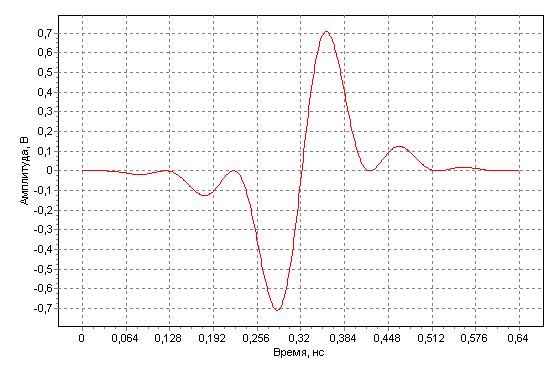
\includegraphics[width=0.7\textwidth]{graphics/tem-horn-vswr-signal}
\caption{СШП импульс, возбуждающий антенну.}
\label{fig:HornAntennaExitationSignal}
\end{figure}

% --- Рисунок
\begin{figure}[p]
\centering
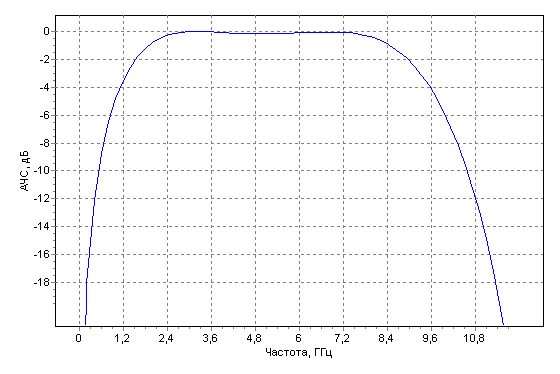
\includegraphics[width=0.7\textwidth]{graphics/tem-horn-vswr-signal-spectrum}
\caption{Амплитудно-частотный спектр импульса на
         рис.~\eqref{fig:HornAntennaExitationSignal}.}
\label{fig:HornAntennaExitationSignalSpectrum}
\end{figure}


% --- Рисунок
\begin{figure}[p]
\centering
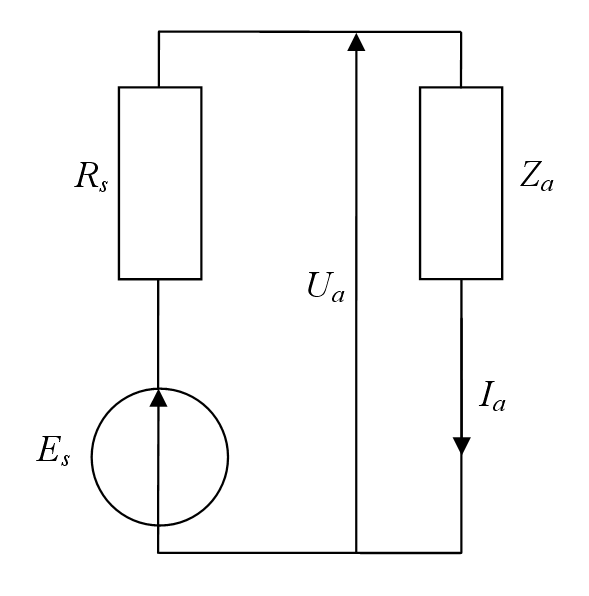
\includegraphics[width=0.3\textwidth]{graphics/horn-equivalent-scheme}
\caption{Эквивалентная схема для расчета волнового сопротивления
         антенны ($R_s=\valu{50}{Ом}$).}
\label{fig:HornAntennaEquivalentScheme}
\end{figure}

% --- Рисунок
\begin{figure}[p]
\centering
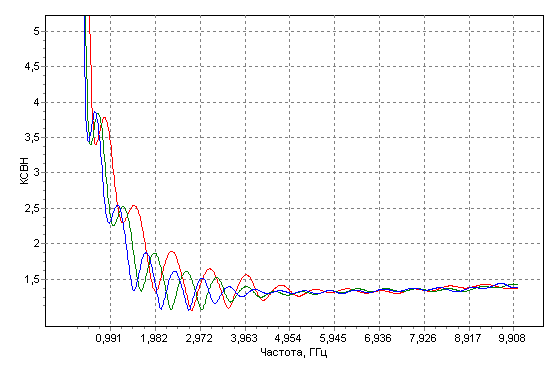
\includegraphics[width=\textwidth]{graphics/horn-vswr}
\caption{Зависимости КСВН от частоты для трех антенн различной длины:
         $R=\valu{150}{мм}$ (красный),
         $R=\valu{180}{мм}$ (зеленый)
       и~$R=\valu{200}{мм}$ (синий)}
\label{fig:HornAntennaVSWR}
\end{figure}

% --- Таблица
\begin{table}[tb]
\caption{
    Параметры пространственной сетки и PML, использованные при моделировании
    TEM-рупорных антенн.}
\label{tab:GridParameters}

\newcolumntype{C}{>{\centering\arraybackslash}X}
\begin{tabularx}{\textwidth}{|C|C|C|C|C|}
\hline
    Координата & Шаг, мм & R, \% & Слоев $N$ & Параметр~$g$ \\
\hline
    $x$ & \val{0.50} & \val{0.01} & \val{8} & \val{2.8} \\
    $y$ & \val{0.77} & \val{0.01} & \val{8} & \val{2.6} \\
    $z$ & \val{0.20} & \val{0.01} & \val{8} & \val{31} \\
\hline
\end{tabularx}
\end{table}

% --- Таблица
\begin{table}[tb]
\caption{Расчетные значения граничной частоты для ТЕМ-рупоров.}
\label{tab:ThresholdFrequency}

\newcolumntype{C}{>{\centering\arraybackslash}X}
\begin{tabularx}{\textwidth}{|l|C|C|C|}
    \hline
    \multirow{2}{*}{Уровень КСВН} &
    \multicolumn{3}{c|}{Граничная частота для разных ТЕМ-рупоров, ГГц} \\
    \cline{2-4}
    & $R=\valu{150}{мм}$ & $R=\valu{180}{мм}$ & $R=\valu{200}{мм}$ \\
    \hline
    4 (60\% отражения) & 0,55 & 0,48 & 0,43 \\
    3 (50\% отражения) & 1,05 & 0,88 & 0,80 \\
    2 (33\% отражения) & 1,71 & 1,47 & 1.32 \\
    \hline
\end{tabularx}
\end{table}
